\section{Design}
Conceptualizing a single ETL process as an entity of type \textit{Task}, that is, the ``extraction, transformation and loading of data from a source to destination'', provides a focal point on which the nETL software can be architected. Handling of instances of type \textit{Task} is done by an entity of type \textit{TaskManager}, which for the purposes of nETL v0.1 is implemented as a singleton (many instances of \textit{TaskManager} could potentially be useful if scaling of nETL were required). Objects of type \textit{Task} are instantiated via a \textit{Task} constructor, which takes a configuration object as an argument. This configuration is specified as a JSON file in which an operation of type \textit{Extraction}, operation(s) of type \textit{Transformation} and an operation of type \textit{Load} is described.

Starting the long-running nETL process comprises instantiating the singleton instance of type \textit{App}. This object holds references to the singleton instance of \textit{TaskManager} (taskManager), the E, T, and L operations and provides a CLI (command line interface) to facilitate user interactions. Via the CLI, users can interact with taskManager and load custom E, T, and L operations as well as start/stop tasks, configure application options such as log output path, etc. Via the CLI, the taskManager object is also able to provide user-feedback on the progress of tasks, messages from the E, T, and L operations, as well as display any program faults that may occur.

E, T, and L operations consist of JavaScript modules executable functions) that should adhere to their respective contracts; specifically, the contracts stipulate an object return on invocation of the module that creates closure over a variety of functions that can then be invoked by taskManager according to the required operation specified by the task object.

\begin{figure}[H]
    \centering
    \begin{mdframed}
        \centering
        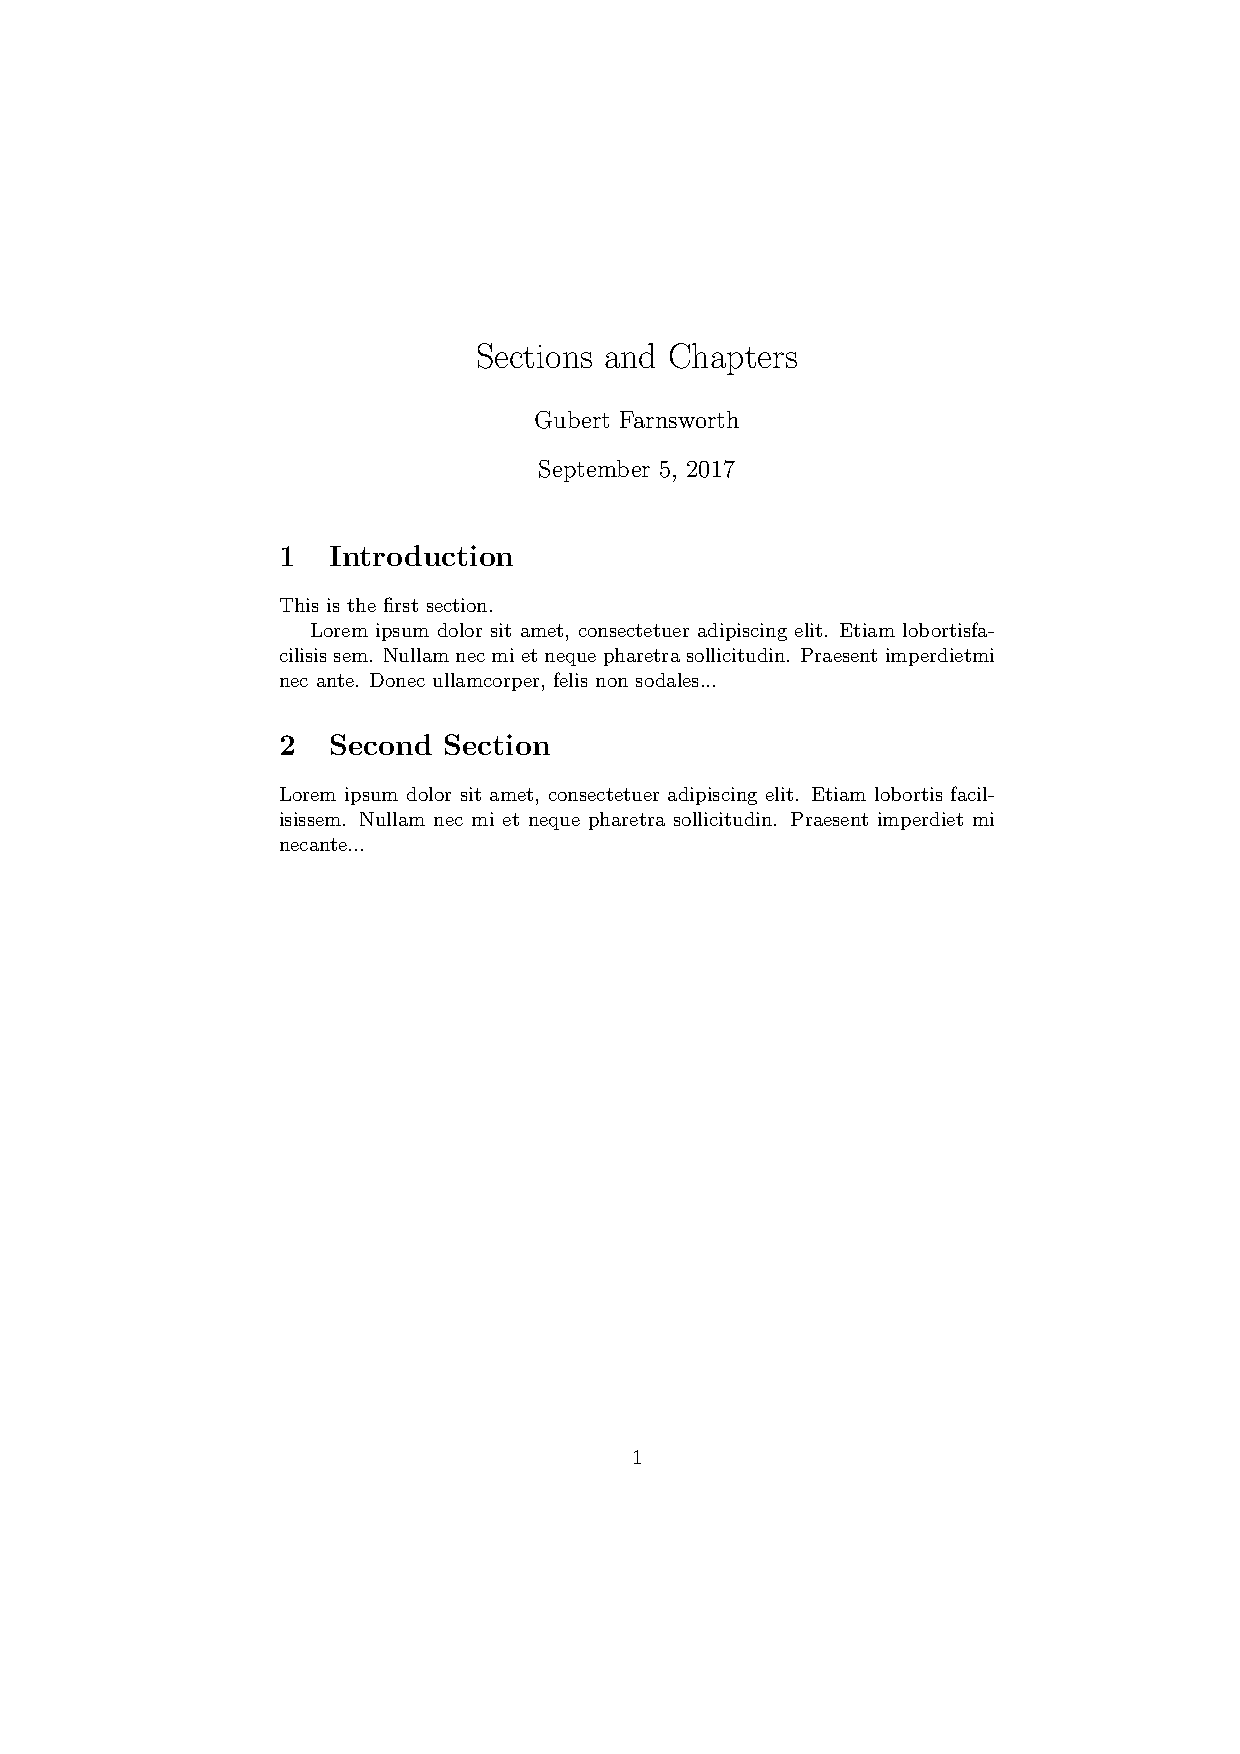
\includegraphics[scale=0.39]{./resources/figures/netl.png}
    \end{mdframed}
    \caption[nETL Architecture]{\textbf{Figure \ref{nETL}: nETL Architecture.} \textit{nETL} is an ETL framework designed to host user-created \textit{Modules} to define \textit{extraction}, \textit{transformation} and \textit{loading} processes. \textit{Modules}, shown in the colored boxes, consist of two parts: a configuration object (a JSON object) and a function that adheres to the specified contract. On startup the \textit{nETL} framework loads modules via the operations via a function made available by the main class. The modules are then cached in main memory by the \textit{nETL} process. A user can then interact with the TaskManager class to create a new task via loading a JSON configuration that makes use of a particular \textit{Module}. Tasks consist of an \textit{Extraction module} configuration, several \textit{Transformation module} configurations and a \textit{Load} configuration. Because modules are created and defined by users, as well as the order in which modules are executed, input/output contracts are also defined by the user, and as such \textit{ETL} processes are infinitely configurable.}
    \label{nETL}
\end{figure}

Figure \ref{nETL} shows the architecture for a configurable component-based ETL tool, including both the application framework and the E, T, and L operations components. JavaScript is a suitable language to prototype this application for a number of reasons:

\begin{itemize}
    \item It has a very succinct API making it fast to write code in (i.e. it is a highly abstracted language similarly to Ruby or Python)
    \item But unlike Ruby or Python (and other high level languages), it is opinionated in that it handles IO asynchronously by default
    \item The JavaScript implementation of object-orientation is appealing (to some developers at least \cite{xxx})
    \item JavaScript is very much in line with the spirit of CouchDB
\end{itemize}